\begin{tikzpicture}[transform shape,scale=0.75]
    \draw (1.5,0.5) node[above right] {File contents};
\only<-4,7>{
    \node (d1) at (2,0) [draw,minimum width=1cm,minimum height=1cm] {data};
    \node (d2) at (3,0) [draw,minimum width=1cm,minimum height=1cm] {data};
}
    \node (d3) at (4,0) [draw,minimum width=1cm,minimum height=1cm] {data};
    \node (d4) at (5,0) [draw,minimum width=1cm,minimum height=1cm] {data};
    \node (d5) at (6,0) [draw,minimum width=1cm,minimum height=1cm] {data};
    
\only<3->{
    \node (p1) at (7,0) [blue,draw,minimum width=1cm,minimum height=1cm] {\footnotesize parity};
    \node (p2) at (8,0) [blue,draw,minimum width=1cm,minimum height=1cm] {\footnotesize  parity};
}
    
    \node (algo) at (6.5,-3) [above right,minimum width=1cm,minimum height=1cm,draw,fill=black!10,node contents={algorithm}] {};

\only<2-3>{
    \draw[->,>=stealth,out=270,in=180] (d1.south) to (algo.west);
    \draw[->,>=stealth,out=270,in=180] (d2.south) to (algo.west);
    \draw[->,>=stealth,out=270,in=180] (d3.south) to (algo.west);
    \draw[->,>=stealth,out=270,in=180] (d4.south) to (algo.west);
    \draw[->,>=stealth,out=270,in=180] (d5.south) to (algo.west);
}
\only<3>{
    \draw[->,>=stealth,out=90,in=270] (algo.north) to (p1.south);
    \draw[->,>=stealth,out=90,in=270] (algo.north) to (p2.south);
}
    
\only<6-7>{
    \draw[->,>=stealth,out=270,in=90] (d3.south) to (algo.north);
    \draw[->,>=stealth,out=270,in=90] (d4.south) to (algo.north);
    \draw[->,>=stealth,out=270,in=90] (d5.south) to (algo.north);
    \draw[->,>=stealth,out=270,in=90] (p1.south) to (algo.north);
    \draw[->,>=stealth,out=270,in=90] (p2.south) to (algo.north);
}
\only<7>{
    \draw[->,>=stealth,out=180,in=270] (algo.west) to (d1.south);
    \draw[->,>=stealth,out=180,in=270] (algo.west) to (d2.south);
}
\end{tikzpicture}
